% !TEX encoding = UTF-8
% !TEX TS-program = pdflatex
% !TEX root = ../../tesi.tex

\section{Smart contract per Ethereum}
Lo \textit{smart contract} per Ethereum ha il compito di gestire gli NFT generati dalla piattaforma NFTLab nella \textit{blockchain} Ethereum.

\subsection{Progettazione}
A partire da quanto richiesto dall'analisi dei requisiti, ho basato la soluzione progettuale dello \textit{smart contract} per Ethereum sulle \textit{best practies} e le convenzioni del linguaggio Solidity, così da limitare il più possibile il consumo di \textit{Gas} e garantire la sicurezza del contratto. \\

\noindent Per quanto concerne i \textit{design pattern}, sono stati utilizzati:
\begin{itemize}
  \item \textbf{\textit{Guard Check}}: facente parte dei \textit{pattern} comportamentali, consiste nel controllare sia se i dati ricevuti in \textit{input} da una funzione siano corretti e sia se, in determinate parti, lo stato del contratto è quello aspettato. Si implementa attraverso l'utilizzo della funzione \textit{built-in} chiamata \textit{require};
  \item \textbf{\textit{Access Restriction}}: facente parte dei \textit{pattern} per la sicurezza, consiste nel limitare l'esecuzione di una funzione in base ad una determinata condizione. In questo contratto è stato utilizzato per limitare l'accesso alle funzioni di scrittura a solamente il proprietario del contratto, il quale viene impostato durante il \textit{deploy}.
\end{itemize}

\clearpage

\begin{figure}[h!]
  \centering
  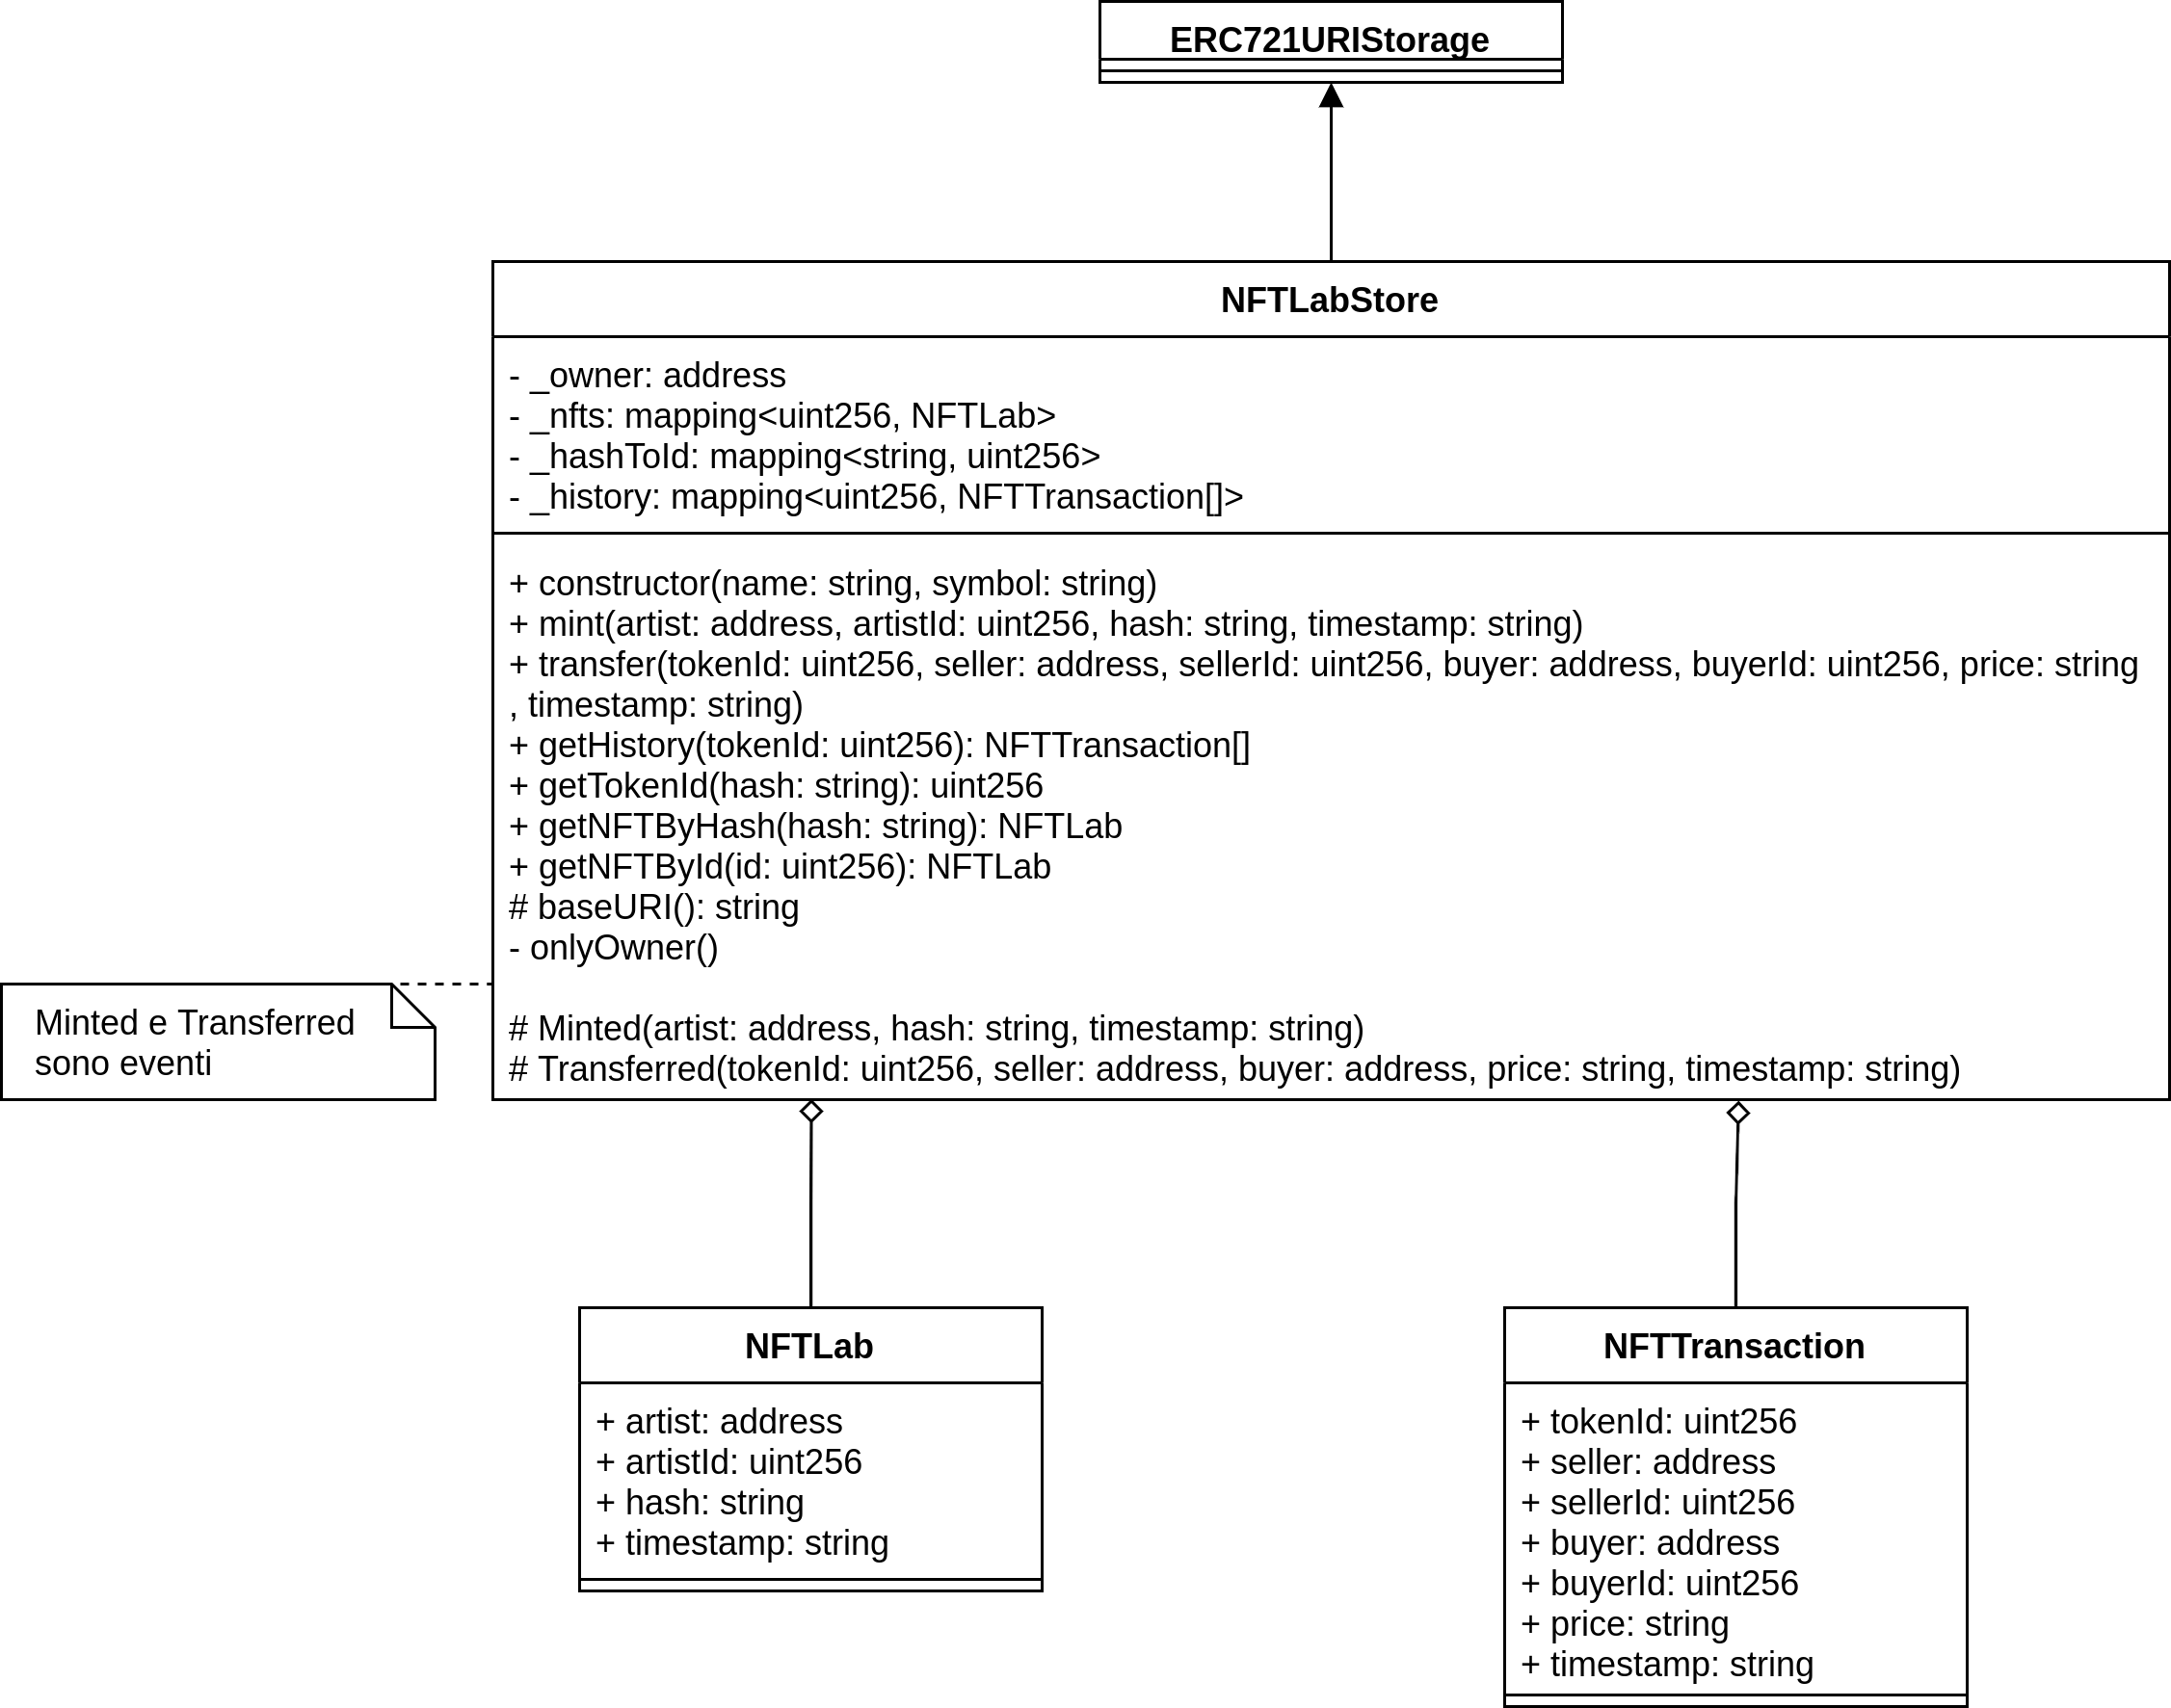
\includegraphics[width=\textwidth]{capitolo3/class-diagram/smart-contract-ethereum-class-diagram.png}
  \caption{Diagramma delle classi dello \textit{smart contract} per Ethereum}
\end{figure}

Il contratto \textit{NFTLabStore} eredita direttamente dal contratto \textit{ERC721URIStorage}, permettendo così anche la memorizzazione del CID di IPFS. Inoltre, sono state utilizzate due strutture dove andare a memorizzare i dati del NFT e delle transazioni. Dato che per l'integrazione da Java è stata utilizzata la libreria Web3J ho dovuto seguire anche le loro convezioni, in particolare quella dove tutti i metodi che modificano lo stato del contratto non devono ritornare alcun dato.

\subsection{Codifica}
Ultimata la progettazione architetturale dei principali componenti del sistema, è iniziata la fase di codifica nella quale ho semplicemente implementato quanto ottenuto dalla progettazione. Ho sviluppato il contratto scrivendo prima le firme di tutto quello che era richiesto, per poi implementarle. \\

Durante la fase di codifica sono stato molto attento a seguire le \textit{best practices} e le convezioni date dal linguaggio Solidity. In particolare:
\begin{itemize}
  \item tutte le funzioni che non modificano lo stato sono state segnate come \textit{view};
  \item utilizzo di variabili di tipo \textit{memory} per tutti gli oggetti che non devono essere memorizzati.
\end{itemize}

% \clearpage

% \begin{figure}[h!]
%   \centering
%   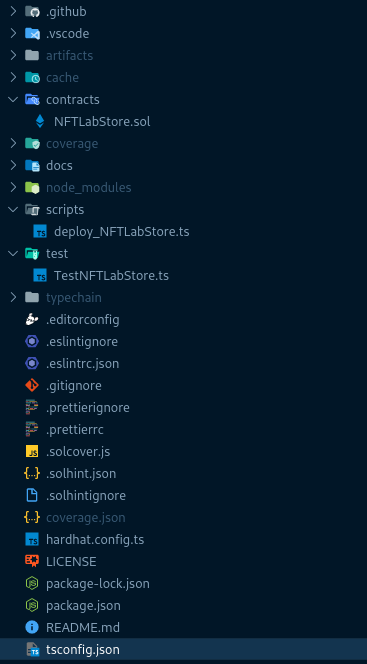
\includegraphics[width=0.3\textwidth]{capitolo3/smart-contract-ethereum/smart-contract-ethereum-structure.png}
%   \caption{Struttura del progetto del contratto per Solidity}
% \end{figure}

Meritevole di attenzione è sicuramente l'implementazione del \textit{design pattern \textbf{Access Restriction}}. Come si può vedere nel costruttore viene assegnata una variabile, la quale specifica che chi ha eseguito il \textit{deploy} del contratto è il proprietario. In seguito viene creato un modificatore che permette di limitare l'esecuzione di determinate funzioni solo al proprietario.

\begin{figure}[h!]
  \centering
  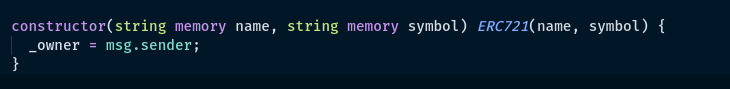
\includegraphics[width=0.8\textwidth]{capitolo3/smart-contract-ethereum/smart-contract-ethereum-constructor.png}
  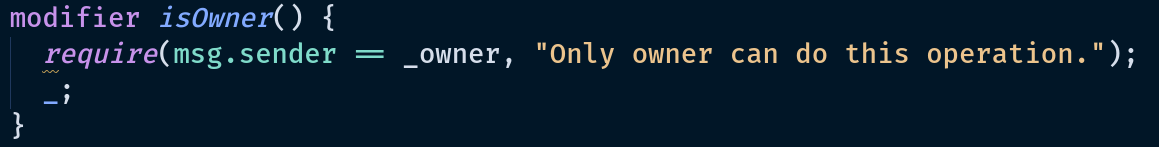
\includegraphics[width=0.8\textwidth]{capitolo3/smart-contract-ethereum/smart-contract-ethereum-modifier.png}
  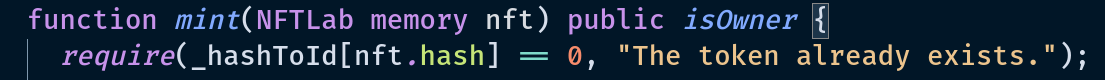
\includegraphics[width=0.8\textwidth]{capitolo3/smart-contract-ethereum/smart-contract-ethereum-modifier-usage.png}
  \caption{Realizzazione del \textit{design pattern Access Restriction} in Solidity}
\end{figure}

\subsection{Verifica}
In parallelo con l'attività di codifica, ho verificato lo sviluppo del contratto sfruttando il \textit{framework} \textbf{Mocha} e la libreria \textbf{Chai}. Questi ultimi si integrano perfettamente con lo strumento HardHat, permettendo la scrittura di tutti questi test attraverso il linguaggio Typescript. Dato che lo \textit{smart contract} può essere eseguito solamente su \textit{blockchain}, HardHat provvederà ad eseguire il \textit{deploy} di quest'ultimo in una \textit{blockchain} temporanea dove verranno eseguiti tutti i \textit{test}. Questo avviene tramite una libreria ed uno strumento aggiuntivo per HardHat, ovvero Ether.js e \textit{Typechain}. HardHat, durante la fase di compilazione, genera automaticamente gli ABI del contratto che \textbf{\textit{Typechain}}, in fase di test, utilizzerà per la generazione di file Typescript che hanno il compito di interagire, grazie a \textbf{Ether.js}, con il contratto caricato. In seguito questi \textit{file} verranno richiamati per eseguire e verificare le varie parti del contratto. \\

Per quanto riguarda i tipi di \textit{test} eseguiti, gli unici che sono stati sviluppati sono quelli di unità, perché non potevano essere sviluppati altri tipi di \textit{test} per la natura semplice delle funzioni del contratto.

\clearpage
\begin{figure}[h!]
  \centering
  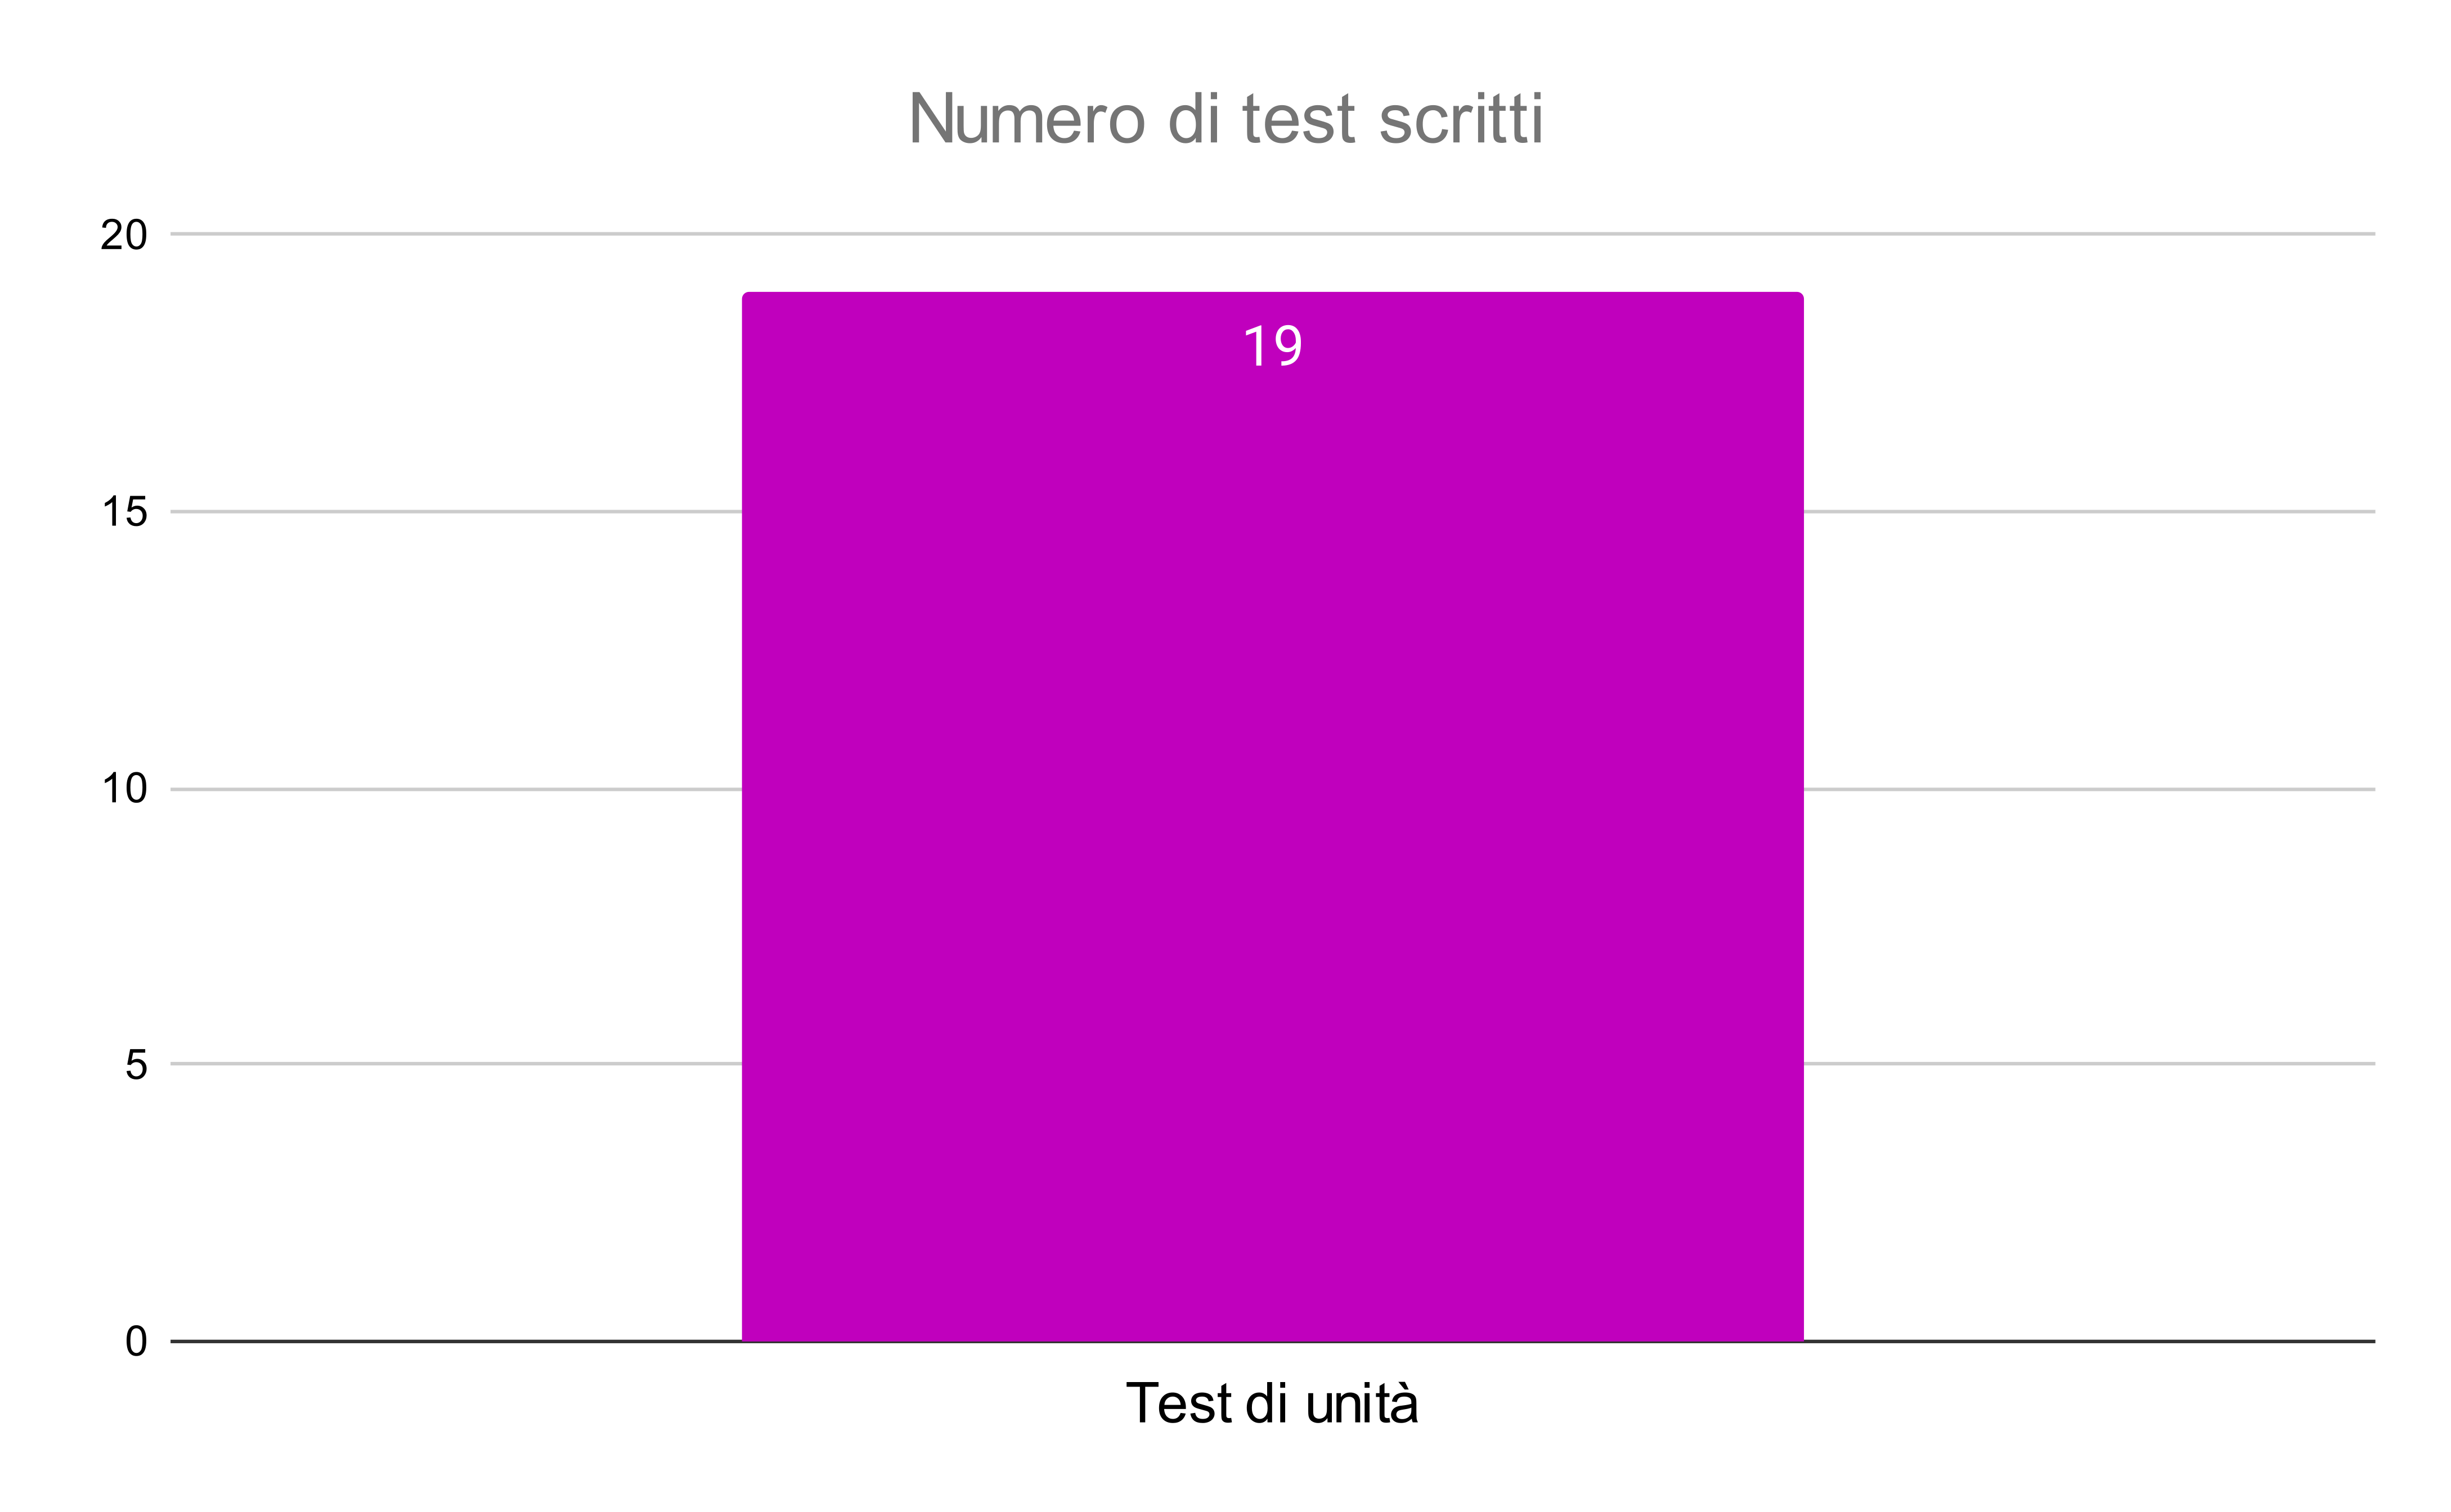
\includegraphics[width=0.9\textwidth]{capitolo3/smart-contract-number-test.png}
  \caption{Numero di \textit{test} scritti nel contratto in Ethereum}
\end{figure}

In generale, posso affermare che l'attività di verifica si è rilevata molto proficua e mi ha permesso di agevolare lo sviluppo in modo significativo, tanto da produrre un grande quantitativo di \textit{test} e raggiungere un \textit{code coverage} del 100\%.

\begin{figure}[h!]
  \centering
  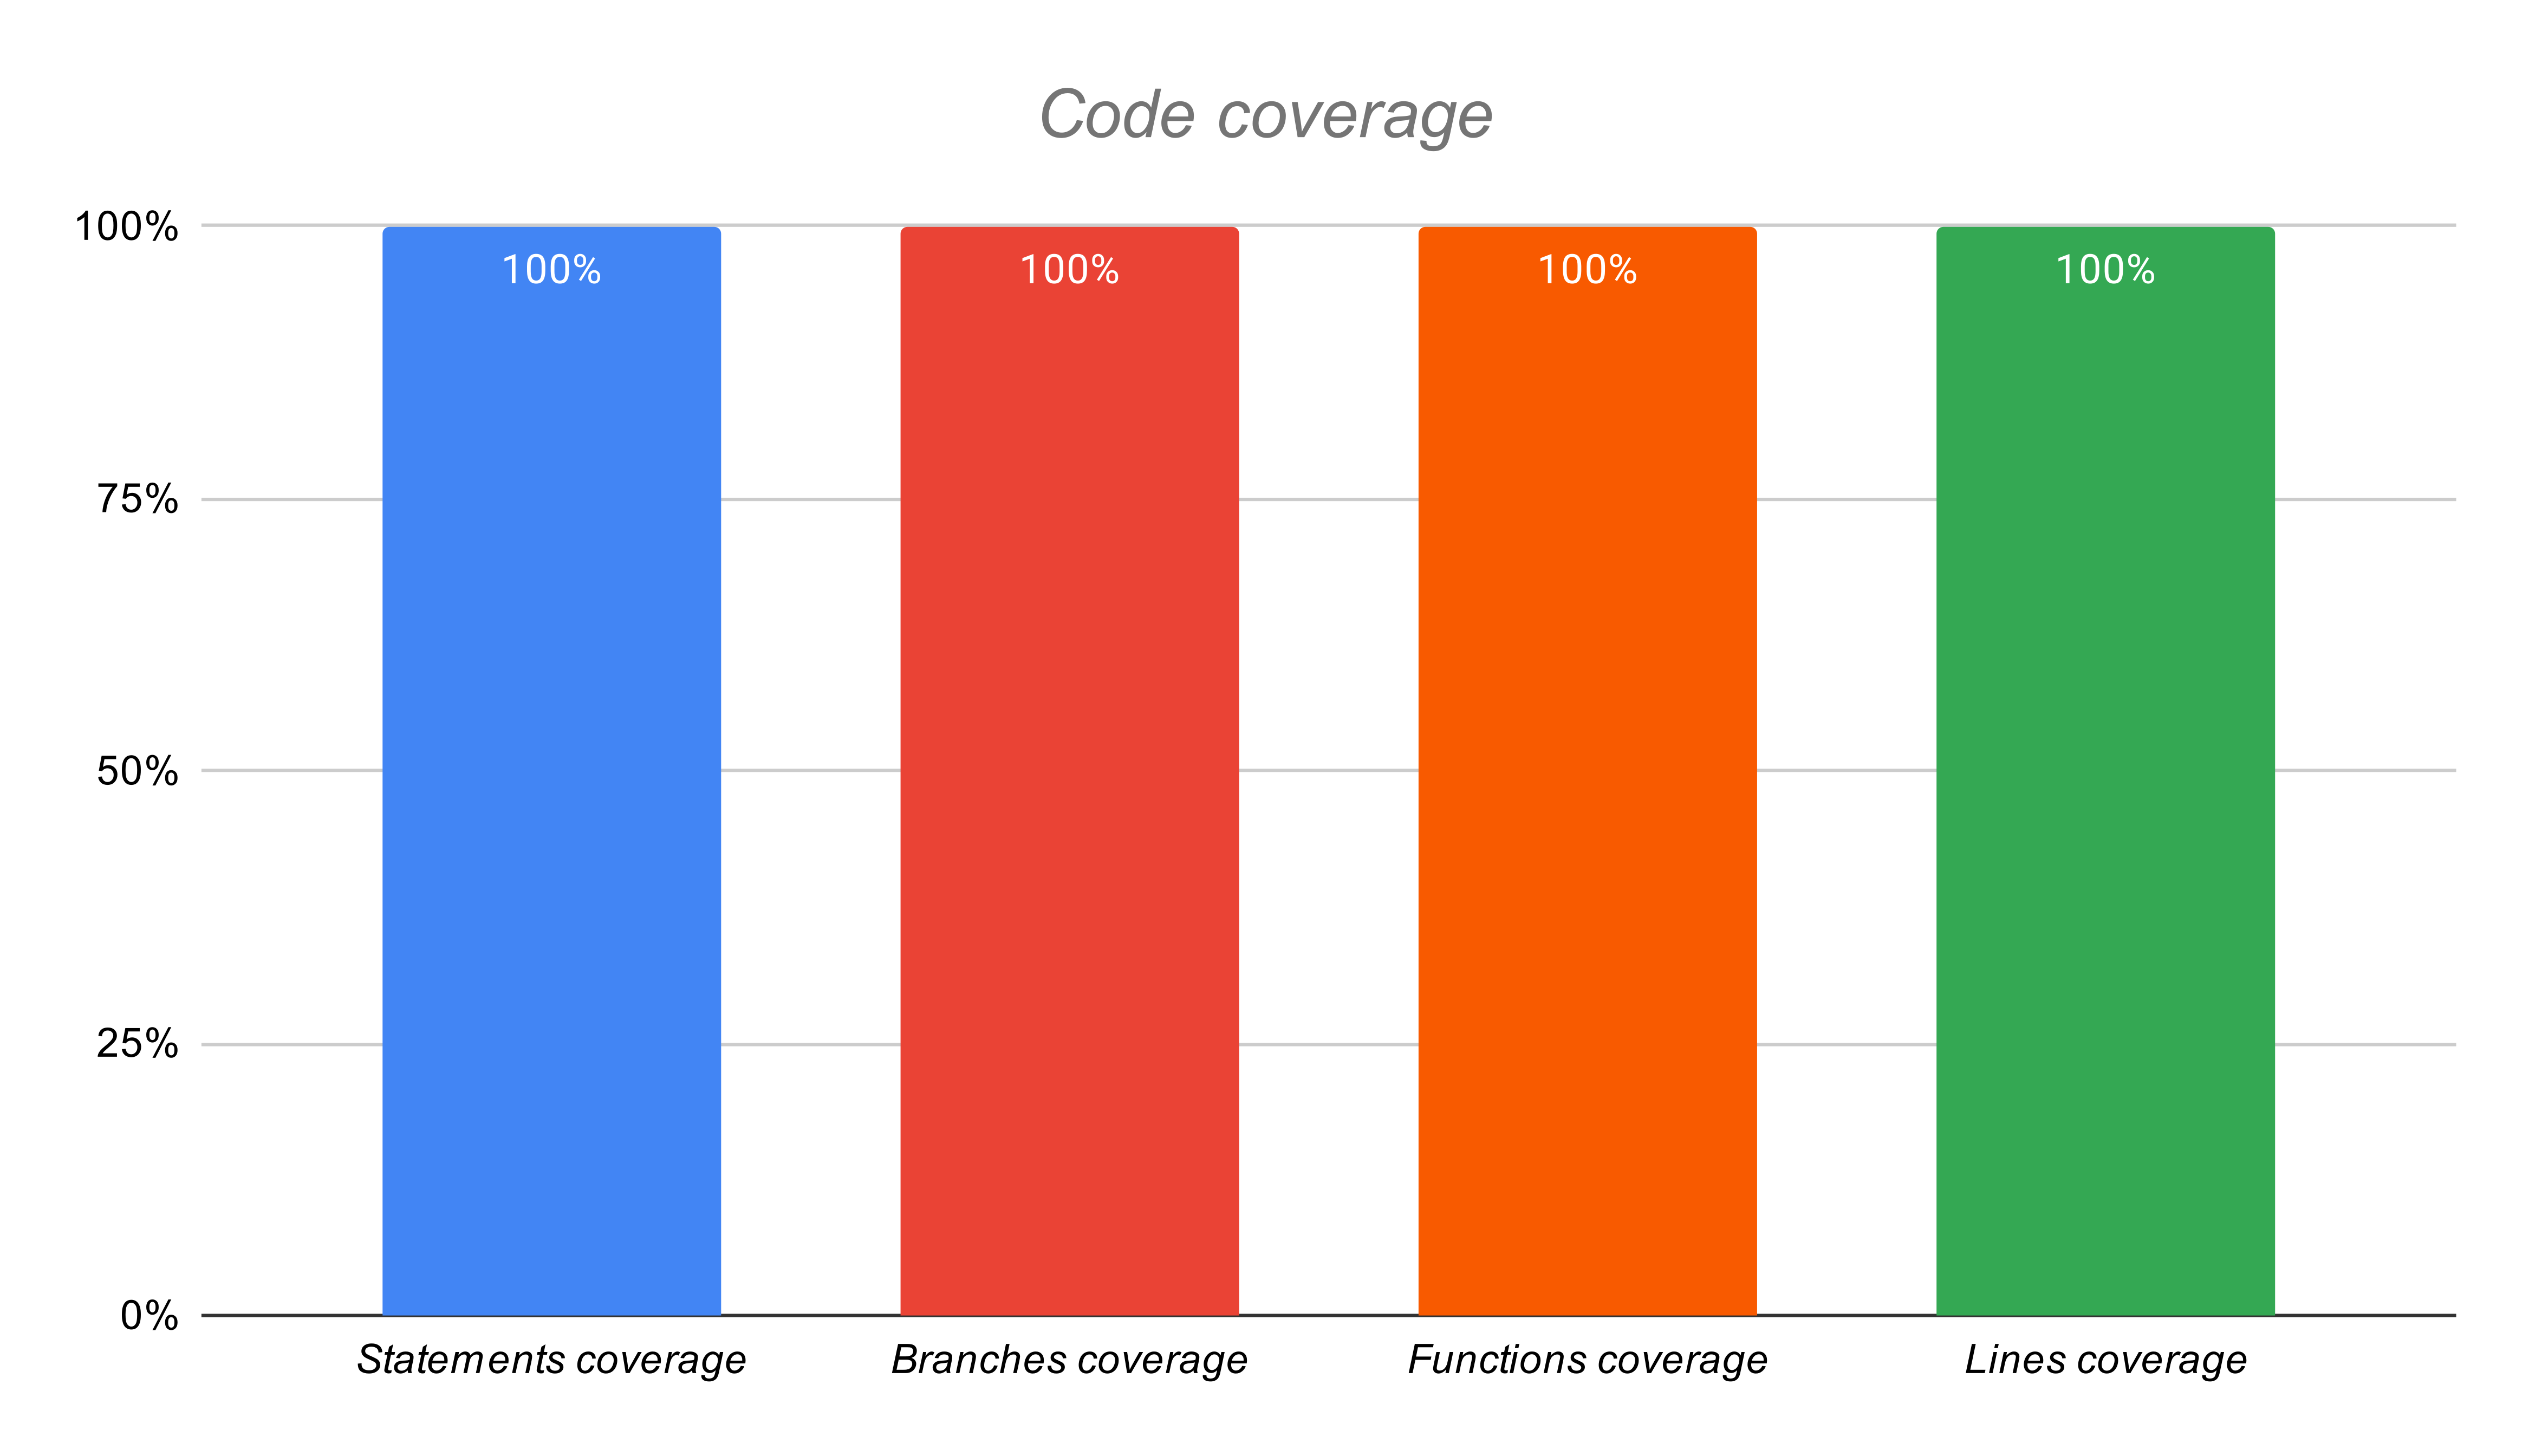
\includegraphics[width=0.9\textwidth]{capitolo3/smart-contract-code-coverage.png}
  \caption{\textit{Code coverage} raggiunto nel contratto in Ethereum}
\end{figure}
